\documentclass{beamer}

\usepackage[utf8]{inputenc}
\usepackage[english]{babel}
\usepackage{graphicx}
\usepackage{color}
\usepackage{natbib}
\usepackage{amssymb}
\usepackage{algorithm}
\usepackage{algpseudocode}
\usepackage{caption}

\usepackage{amsmath}
\usepackage{tikz}
\usetikzlibrary{arrows,calc,tikzmark,shapes.misc}

\tikzset{every picture/.style=remember picture}
% Define a TikZ node for math content:
\newcommand{\mathnode}[2]{%
  \mathord{\tikz[baseline=(#1.base), inner sep = 0pt]{\node (#1) {$#2$};}}}

\DeclareMathOperator*{\argmin}{arg\,min}
\DeclareMathOperator*{\argmax}{arg\,max}


% Beamer layout
\hypersetup{colorlinks=True, citecolor=green, linkcolor=blue}

\let\oldbibitem=\bibitem
\renewcommand{\bibitem}[2][]{\label{#2}\oldbibitem[#1]{#2}}
\let\oldcite=\cite
\renewcommand\cite[1]{\hyperlink{#1}{\oldcite{#1}}}
\let\oldcitep=\citep
\renewcommand\citep[1]{\hyperlink{#1}{\oldcitep{#1}}}
\let\oldciteauthor=\citeauthor
\renewcommand\citeauthor[1]{\hyperlink{#1}{\oldciteauthor{#1}}}

\usetheme{boxes}
\beamertemplatenavigationsymbolsempty
\setbeamertemplate{sections/subsections in toc}[circle]
\setbeamertemplate{footline}[frame number]
\setbeamertemplate{itemize items}[circle]
\setbeamertemplate{itemize subitem}[square]

% Front slide
\title{{\bf Bayesian optimisation}}
\author{
Gilles Louppe}
\date{April 11, 2016}

\begin{document}

\begin{frame}[plain]
\titlepage
\centering

\includegraphics[height=1.5em]{nyu.jpg}
\end{frame}

\begin{frame}
    \frametitle{Problem statement}

    \begin{center}
        $$x^* = \arg \max_x f(x)$$
    \end{center}

    \vspace{2em}

    Constraints:
    \begin{itemize}
        \item $f$ is a black box for which no closed form is known;
            \begin{itemize}
                \item gradients $\frac{df}{dx}$ are not available.
            \end{itemize}

        \item $f$ is expensive to evaluate;

        \item (optional) uncertainty on observations $y_i$ of $f$
            \begin{itemize}
                \item e.g., $y_i = f(x_i) + \epsilon_i$ because of Poisson fluctuations.
            \end{itemize}
    \end{itemize}

    \vspace{2em}

    Goal: find $x^*$, while minimizing the number of evaluations $f(x)$.
\end{frame}

\begin{frame}
    \frametitle{\color{red} Disclaimer}
    \begin{center}
        If you do not have these constraints, there is certainly a better optimisation algorithm than Bayesian optimisation.

        \vspace{3em}

        (e.g., L-BFGS-B, Powell's method (as in Minuit), etc)
    \end{center}
\end{frame}

\begin{frame}
    \frametitle{Bayesian optimisation}

    for $t=1:T$,
    \begin{enumerate}
        \item Given observations $(x_i, y_i)$ for $i=1:t$, build a probabilistic model for the objective $f$.
        \begin{itemize}
            \item Integrate out all possible true functions, using
            Gaussian process regression.
        \end{itemize}

        \item Optimise a cheap utility  function $u$ based on the posterior distribution for sampling the next point.
            $$x_{t+1} = \arg \max_x u(x)$$
            Exploit uncertainty to balance exploration against exploitation.

        \item Sample the next observation $y_{t+1}$ at $x_{t+1}$.
    \end{enumerate}

\end{frame}

\begin{frame}
    \frametitle{Where shall we sample next?}

    \begin{center}
        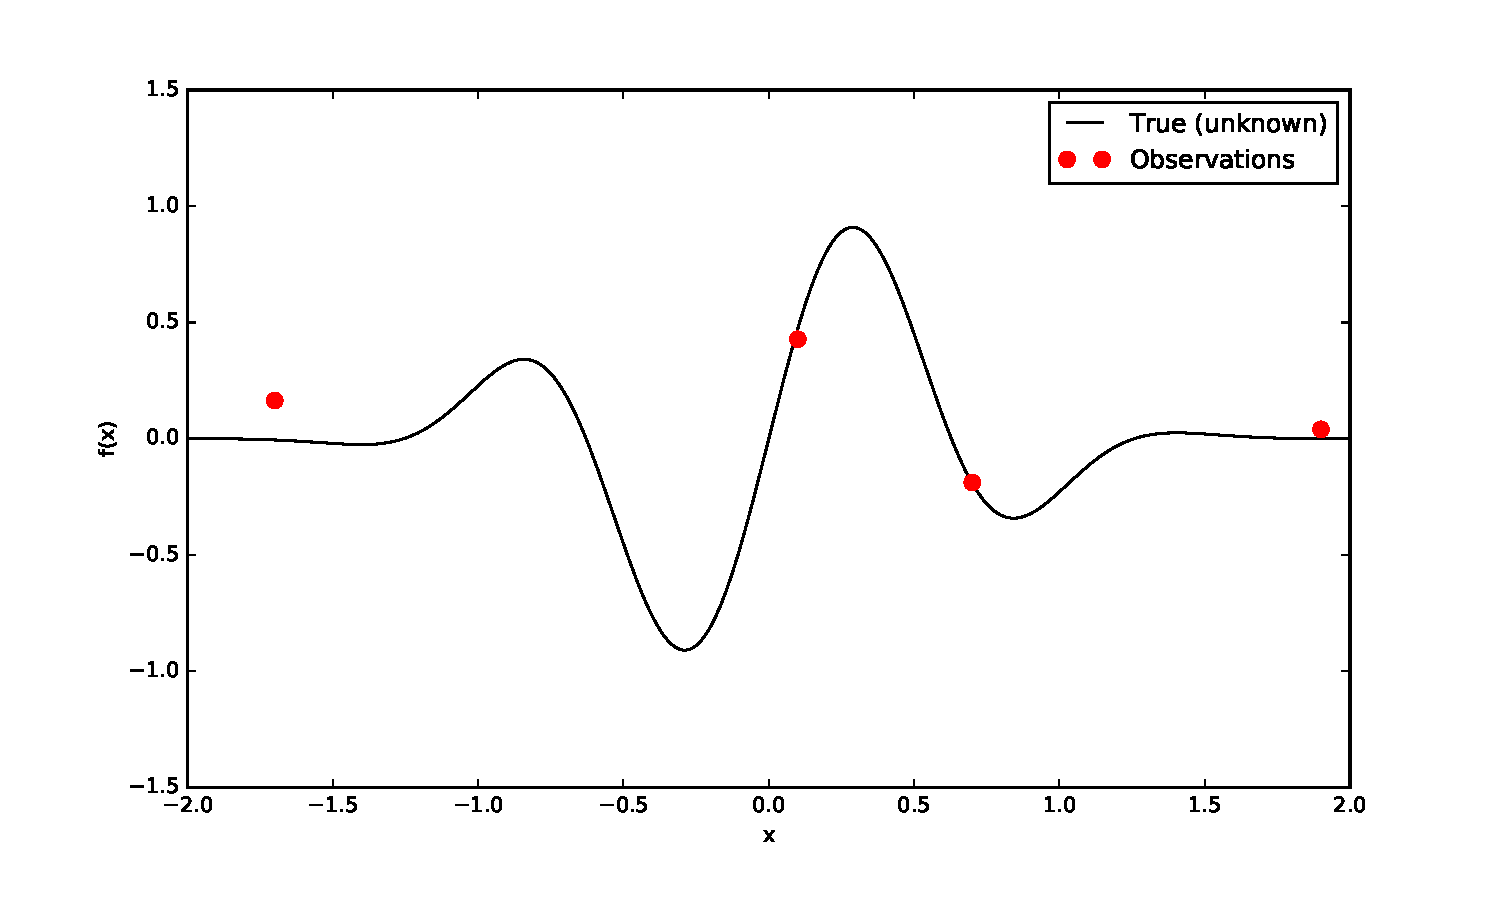
\includegraphics[width=\textwidth]{code/fig1.pdf}
    \end{center}
\end{frame}

\begin{frame}
    \frametitle{Build a probabilistic model for the objective function}
    \begin{center}
        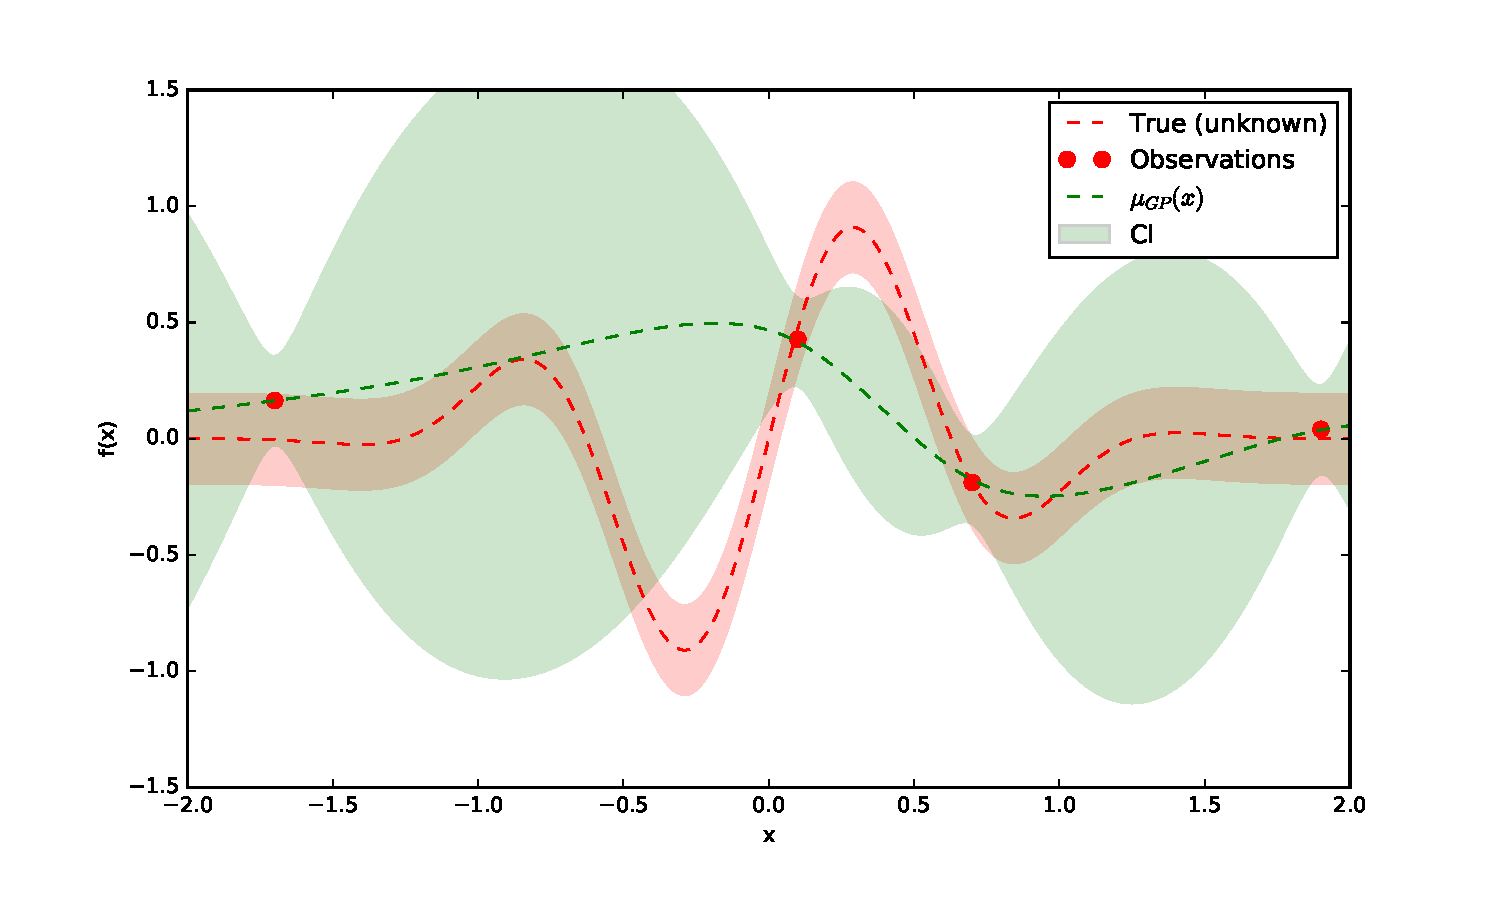
\includegraphics[width=\textwidth]{code/fig2.pdf} \\
        This gives a posterior distribution over functions that could have generated the observed data.
    \end{center}
\end{frame}

\begin{frame}
    \frametitle{Acquisition functions}

    Acquisition functions $\text{u}(x)$ specify which sample $x$ should be tried next:

    \begin{itemize}
        \item Upper confidence bound
            $\text{UCB}(x) = \mu_{GP}(x) + \kappa \sigma_{GP}(x)$;
        \item Probability of improvement
            $\text{PI}(x) = P(f(x) \geq f(x_t^+) + \kappa) $;
        \item Expected improvement
            $\text{EI}(x) = \mathbb{E} [f(x) - f(x_t^+)] $;
        \item ... and many others.
    \end{itemize}

    where $x_t^+$ is the best point observed so far.

    \vspace{1em}

    In most cases, acquisition functions provide knobs (e.g., $\kappa$) for
    controlling the exploration-exploitation trade-off.
        \begin{itemize}
            \item Search in regions where $\mu_{GP}(x)$ is high (exploitation)
            \item Probe regions where uncertainty $\sigma_{GP}(x)$ is high (exploration)
        \end{itemize}

\end{frame}

\begin{frame}
    \frametitle{Plugging everything together ($t=0$)}
    \begin{center}
        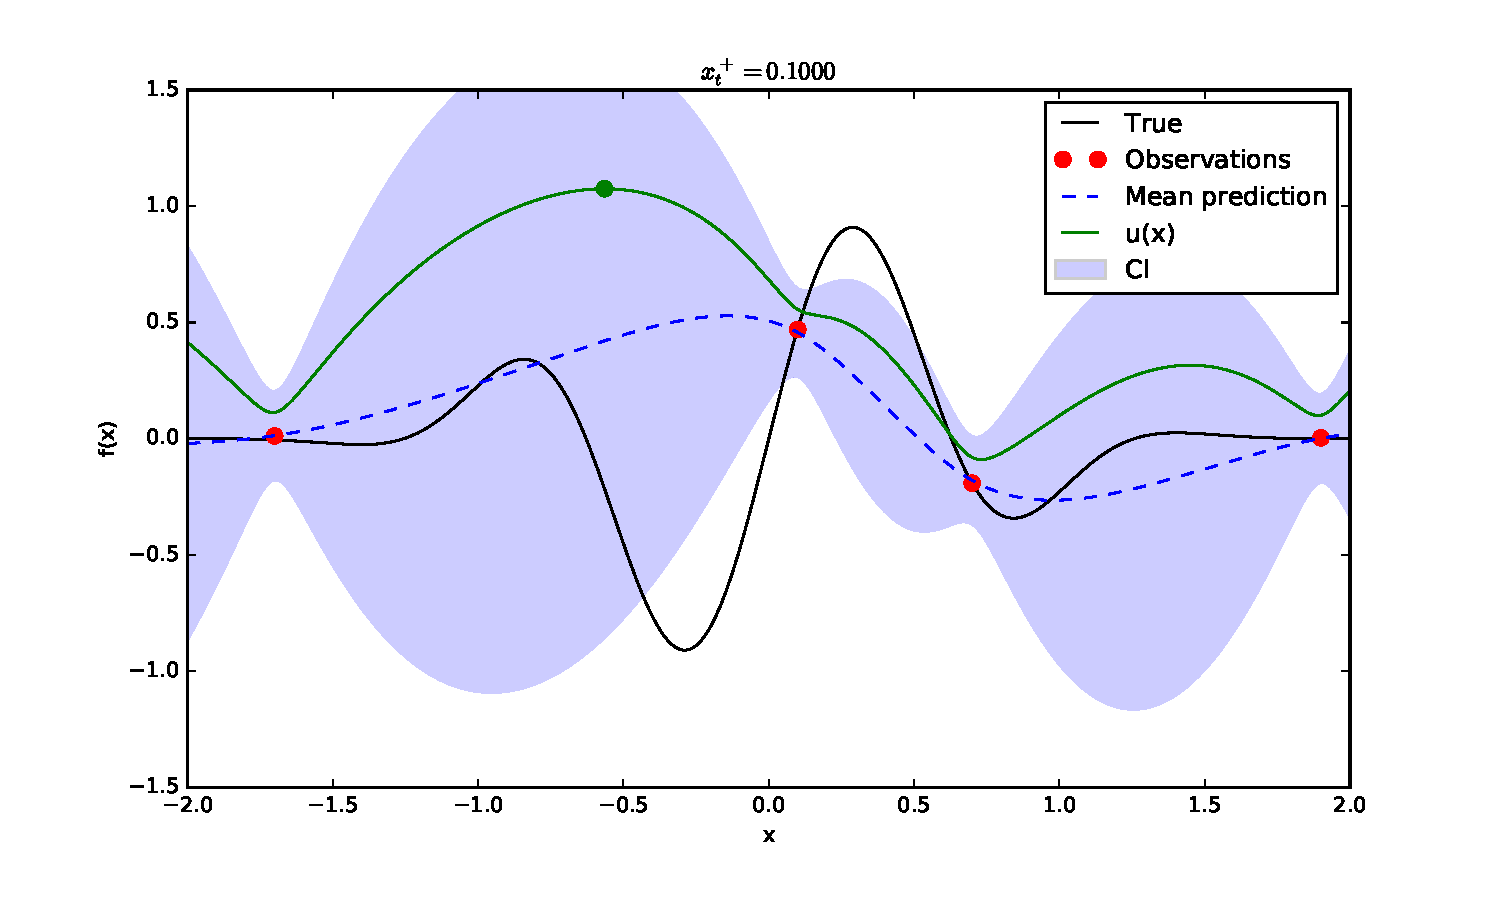
\includegraphics[width=\textwidth]{code/fig4-0.pdf}\\
        $x_{t+1} = \arg \max_{x} \text{UCB}(x)$
    \end{center}
\end{frame}

\begin{frame}
    \frametitle{... and repeat until convergence ($t=1$)}
    \begin{center}
        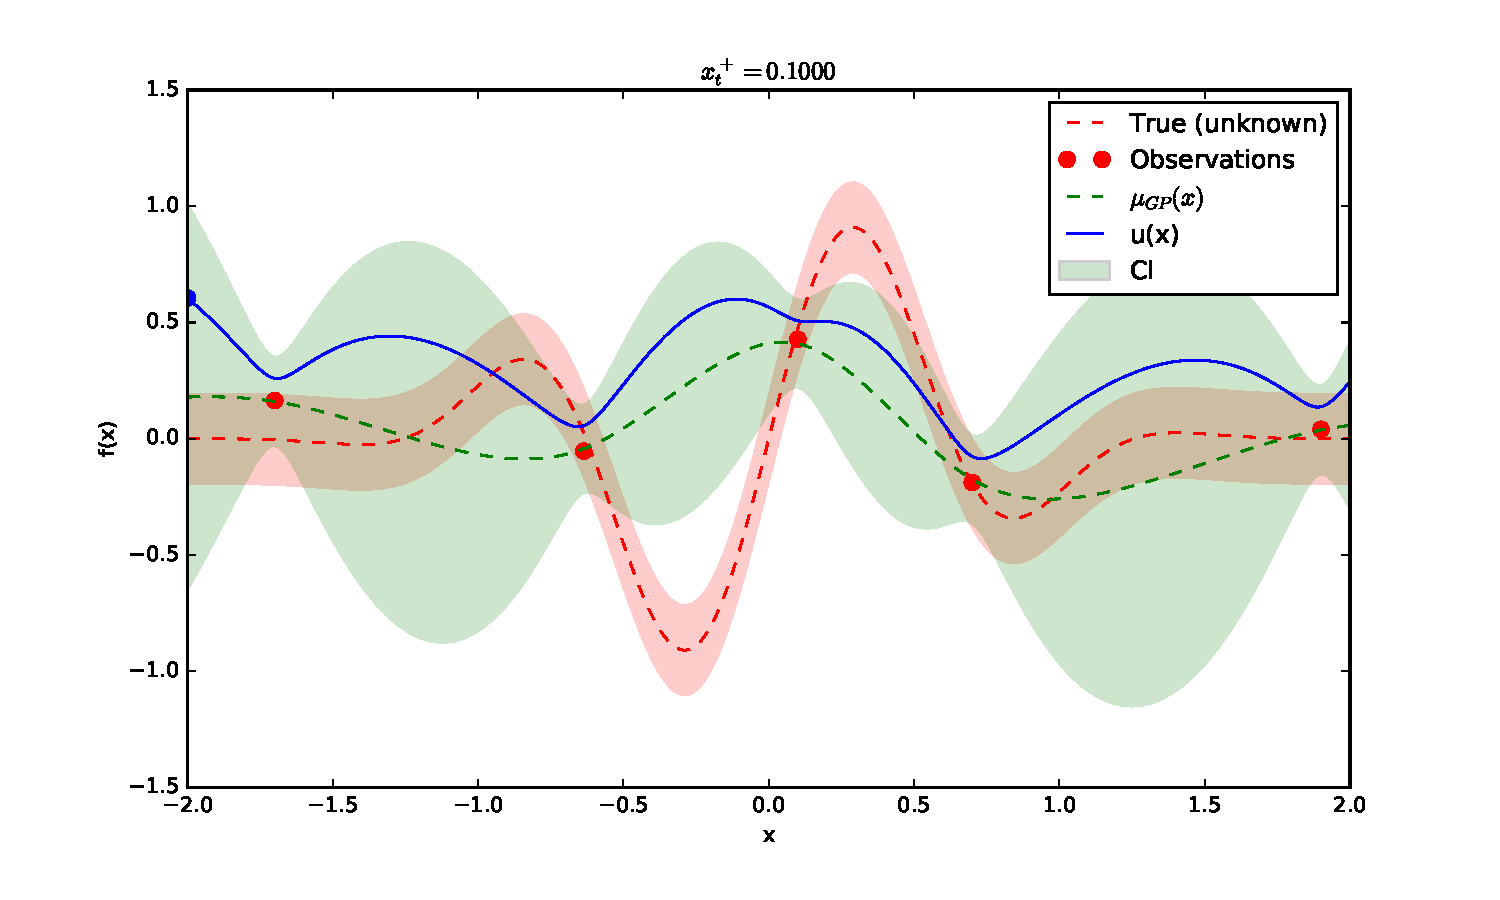
\includegraphics[width=\textwidth]{code/fig4-1.pdf}
    \end{center}
\end{frame}

\begin{frame}
    \frametitle{... and repeat until convergence ($t=2$)}
    \begin{center}
        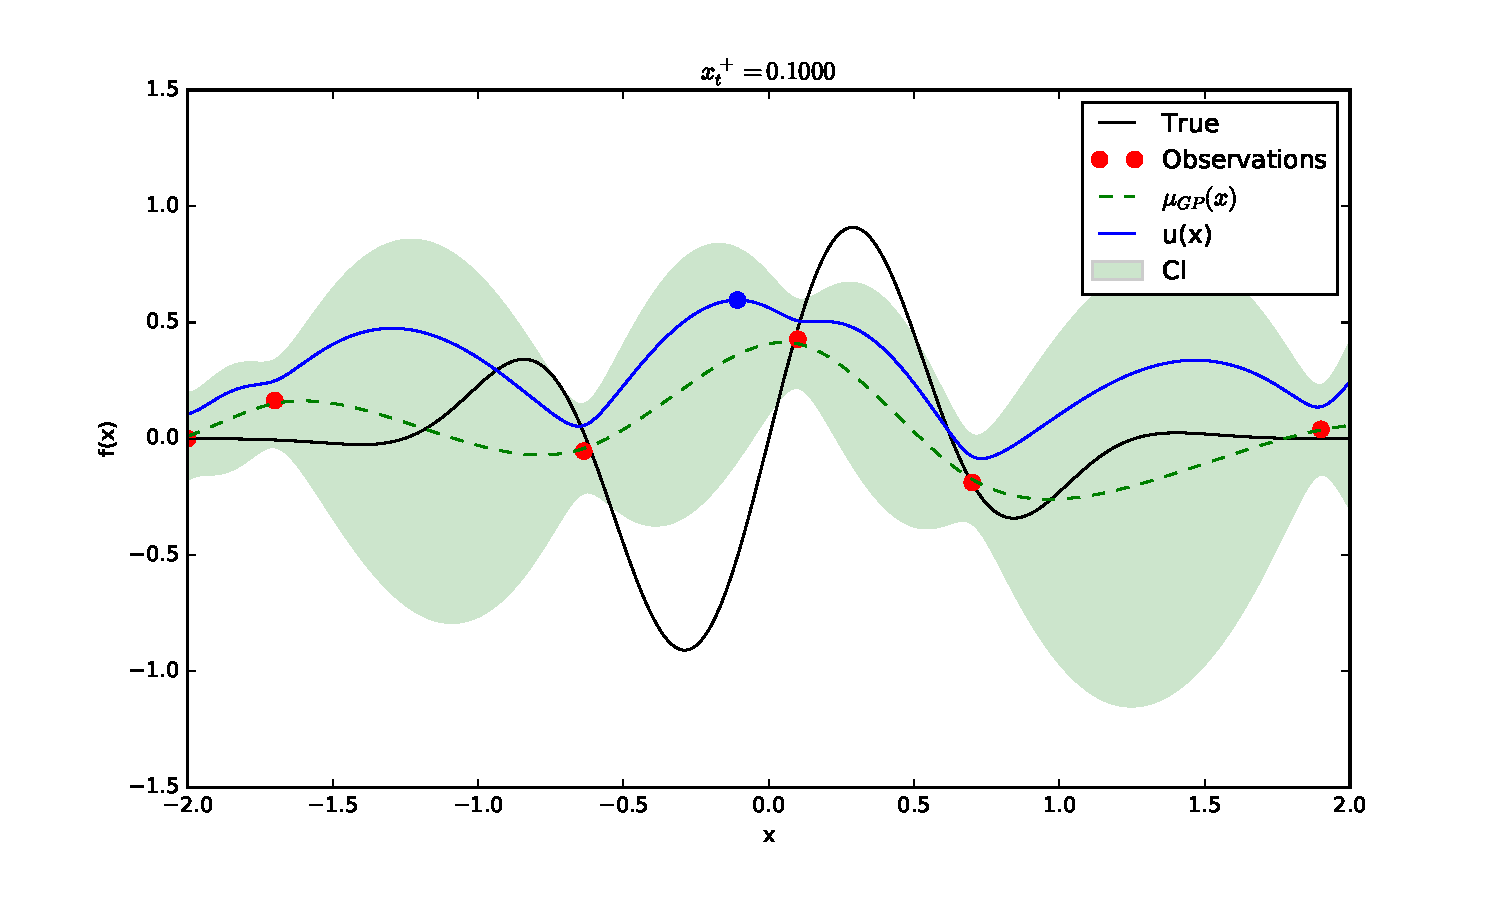
\includegraphics[width=\textwidth]{code/fig4-2.pdf}
    \end{center}
\end{frame}

\begin{frame}
    \frametitle{... and repeat until convergence ($t=3$)}
    \begin{center}
        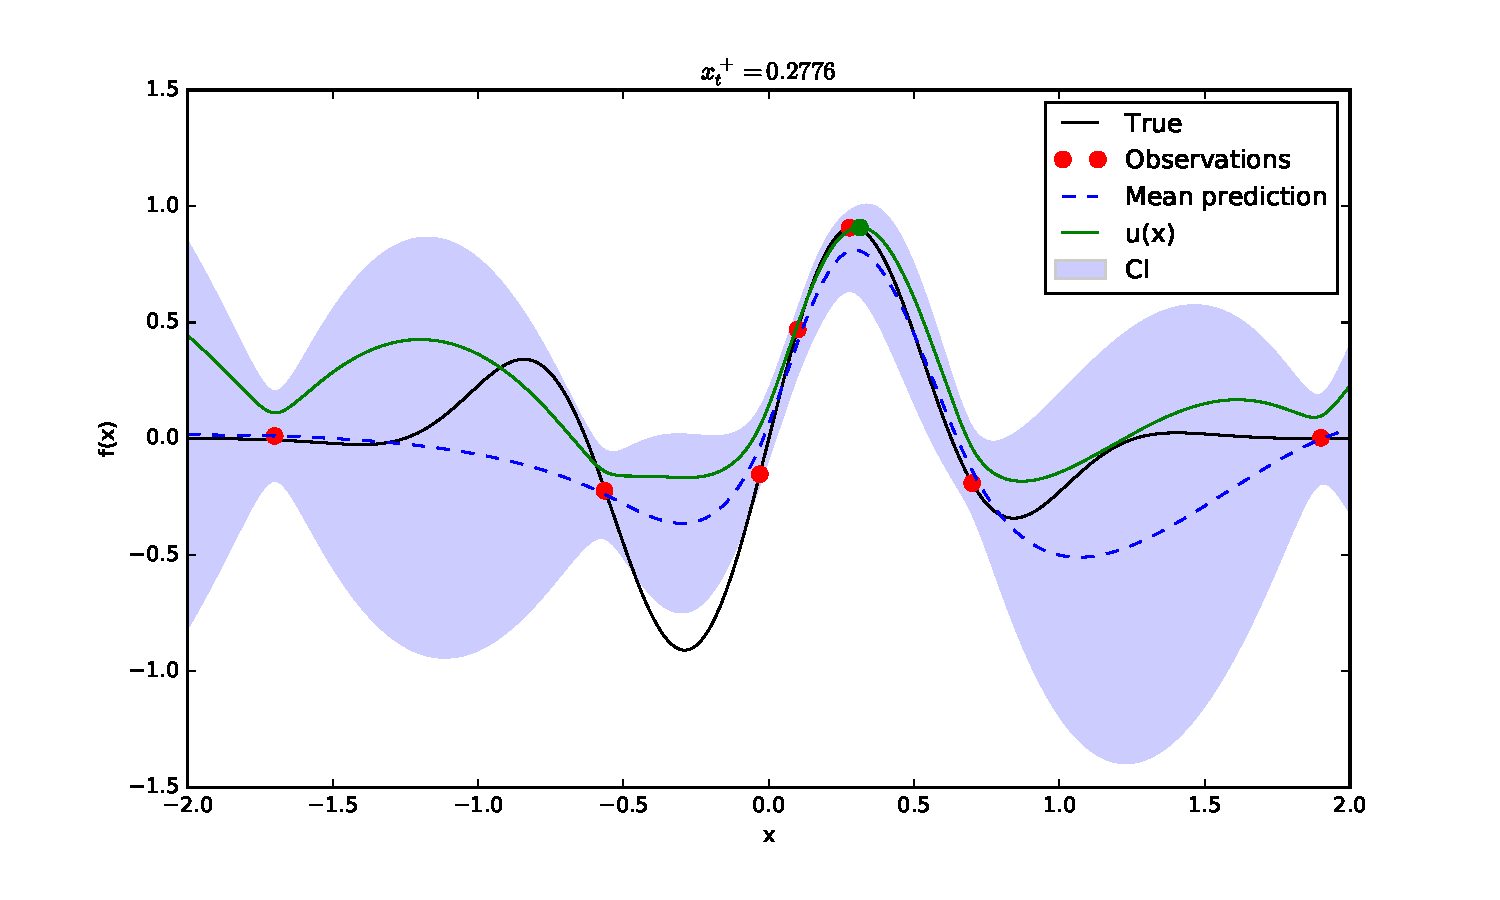
\includegraphics[width=\textwidth]{code/fig4-3.pdf}
    \end{center}
\end{frame}

\begin{frame}
    \frametitle{... and repeat until convergence ($t=4$)}
    \begin{center}
        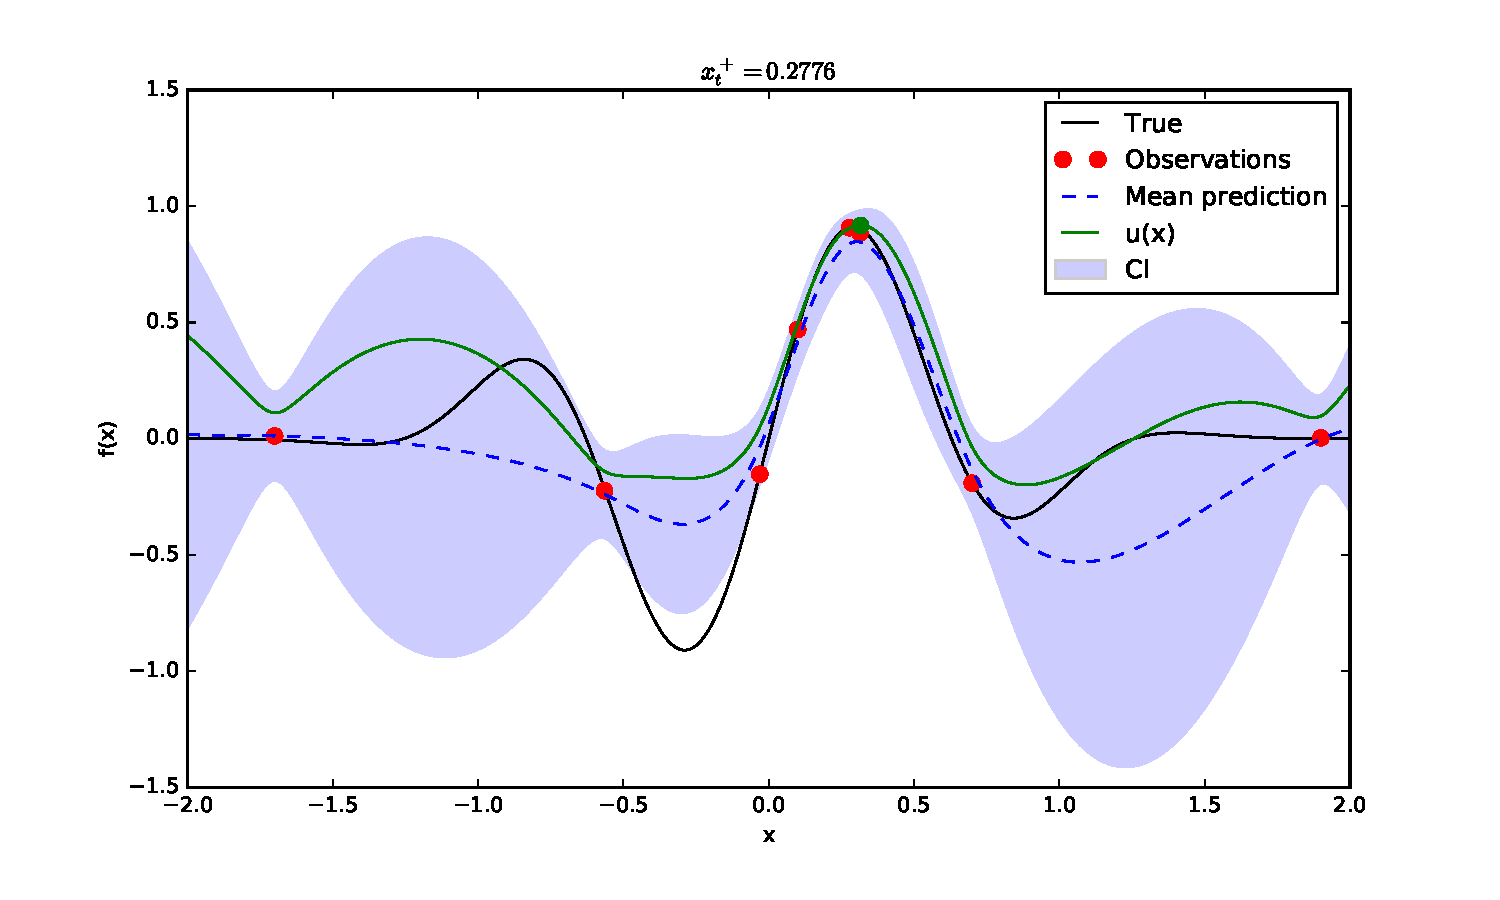
\includegraphics[width=\textwidth]{code/fig4-4.pdf}
    \end{center}
\end{frame}

\begin{frame}
    \frametitle{... and repeat until convergence ($t=5$)}
    \begin{center}
        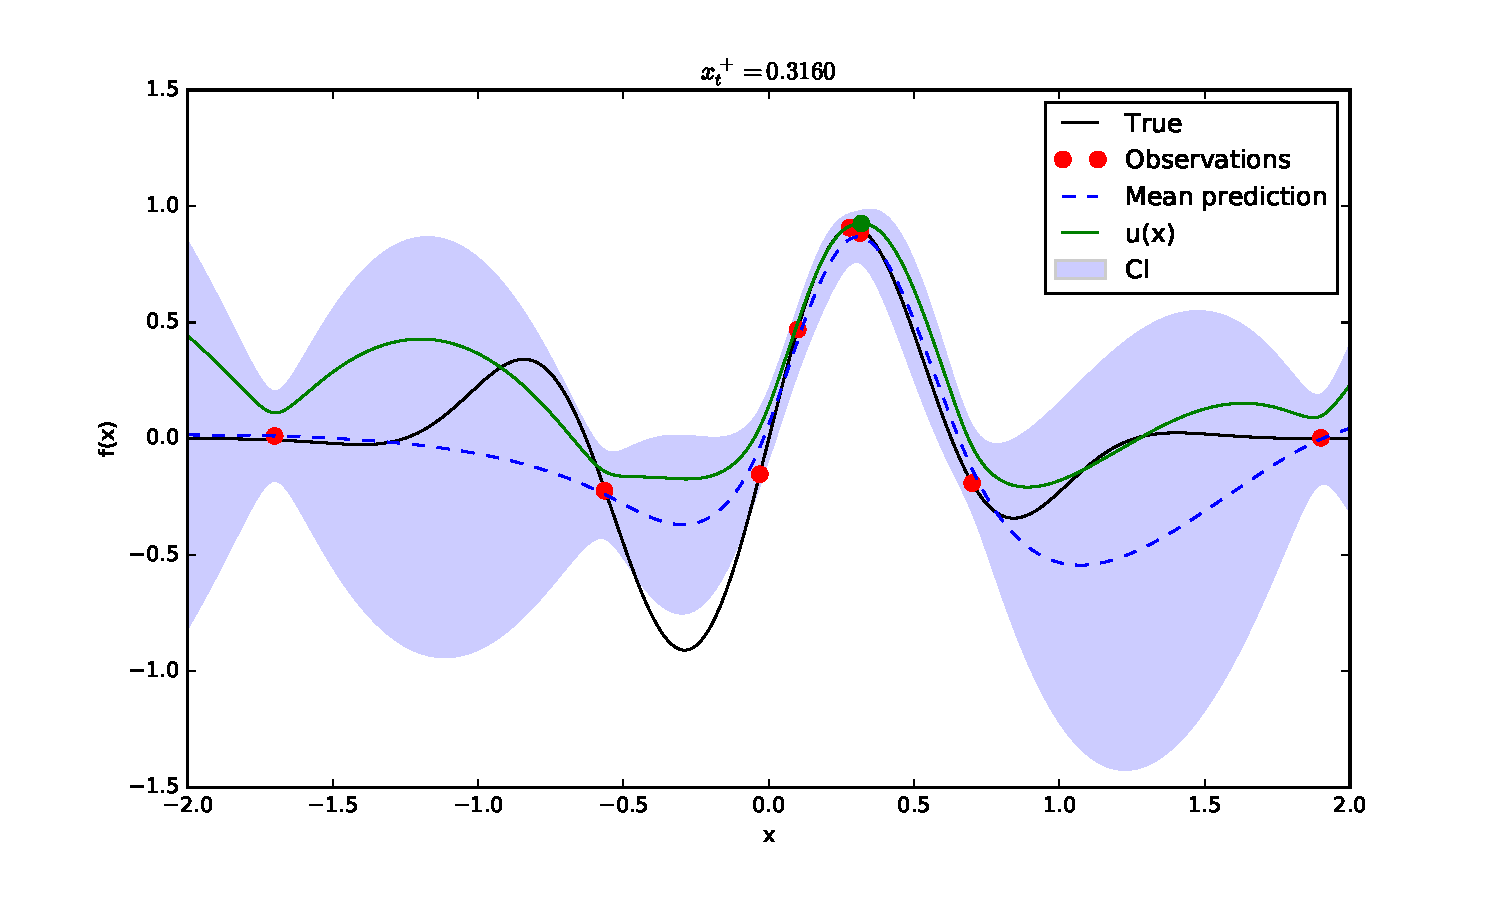
\includegraphics[width=\textwidth]{code/fig4-5.pdf}
    \end{center}
\end{frame}

\begin{frame}
    \frametitle{What is Bayesian about Bayesian optimization?}

    \begin{itemize}
        \item The Bayesian strategy treats the unknown objective function
        as a random function and place a {\it prior} over it.
        \begin{itemize}
            \item The prior captures our beliefs about the behaviour of
            the function. It is here defined by a
            Gaussian process whose covariance function captures assumptions
            about the smoothness of the objective.
        \end{itemize}
        \item Function evaluations are treated as
        data. They are used to update the prior to form the {\it posterior}
        distribution over the objective function.
        \item The posterior distribution, in turn, is used to construct
        an acquisition function for querying the next point.
    \end{itemize}
\end{frame}

\begin{frame}
    \frametitle{Limitations}

    \begin{itemize}
        \item Bayesian optimisation has parameters itself!
            \begin{itemize}
                \item Choice of the acquisition function
                \item Choice of the kernel (i.e. design of the prior)
                \item Parameter wrapping
                \item Initialization scheme
            \end{itemize}

        \vspace{1em}

        \item Gaussian processes usually do not scale well to many observations and to high-dimensional data.
            \begin{itemize}
                \item Sequential model-based optimization provides a direct and effective alternative (i.e., replace GPs by a tree-based model).
            \end{itemize}
    \end{itemize}
\end{frame}

\begin{frame}
    \frametitle{Applications}

    \begin{itemize}
        \item Bayesian optimization has been used in many scientific fields,
        including robotics, machine learning or life sciences.

        \vspace{1em}

        \item Use cases for high energy physics?
            \begin{itemize}
                \item Optimisation of simulation parameters in event generators;
                \item Optimisation of compiler flags to maximize execution speed;
                \item Optimisation of hyper-parameters in machine learning for HEP;
                \item ... let's discuss further ideas?
            \end{itemize}
    \end{itemize}
\end{frame}

\begin{frame}
    \frametitle{Software}

    \begin{itemize}
        \item Python
        \begin{itemize}\scriptsize
            \item Spearmint \url{https://github.com/JasperSnoek/spearmint}
            \item GPyOpt \url{https://github.com/SheffieldML/GPyOpt}
            \item RoBO \url{https://github.com/automl/RoBO}
            \item scikit-optimize \url{https://github.com/MechCoder/scikit-optimize} (work in progress)
        \end{itemize}

        \item C++
        \begin{itemize}\scriptsize
            \item MOE \url{https://github.com/yelp/MOE}
        \end{itemize}
    \end{itemize}

    \vspace{1em}

    \begin{center}
        Check also this \href{https://github.com/glouppe/talk-bayesian-optimisation}{Github} repo for a vanilla implementation reproducing these slides.
    \end{center}

\end{frame}

\begin{frame}
    \frametitle{Summary}

    \begin{itemize}
        \item Bayesian optimisation provides a principled approach for optimising an expensive function $f$;

        \vspace{1em}

        \item Often very effective, provided it is itself properly configured;

        \vspace{1em}

        \item Hot topic in machine learning research. Expect quick improvements!

    \end{itemize}

\end{frame}

\begin{frame}[plain,noframenumbering]
    \frametitle{References}
    \nocite{brochu2010tutorial}
    \nocite{shahriari2016taking}
    {\footnotesize
    \bibliographystyle{apalike}
    \bibliography{biblio}}
\end{frame}

\end{document}
